%%% Template by Mikhail Klassen, April 2013
%%% 
\documentclass[11pt,letterpaper]{article}
\newcommand{\workingDate}{\textsc{2019 $|$ April $|$ 21}}
\newcommand{\userName}{Jordan Sturtz}
\newcommand{\institution}{ Oregon State University}
\usepackage{researchdiary_png}
\usepackage{listings}
\usepackage{amsmath}

% To add your univerisity logo to the upper right, simply
% upload a file named "logo.png" using the files menu above.

\begin{document} \univlogo

\title{CS 475 - Parallel Programming}
{\Huge Project 4 Writeup}\\[5mm]

\begin{enumerate}
  \item \textbf{Machine} 

      I ran these tests on the flip3.oregonstate.edu server by compiling the code with the
        gcc compiler with the -fopenmp flag. 

  \item \textbf{Table and Graph} 
    \begin{lstlisting}
    PERFORMANCE RESULTS
    Size	Mult(No SIMD)	Mult(SIMD)	Reduct(No SIMD)	Reduct(SIMD)
    1000	125.23	        245.93	        130.31	        245.37	    
    2000	162.25	        437.37	        172.07	        439.7	    
    4000	191.28	        718.94	        205.76	        722.82	    
    8000	210.23	        1056.83	        227.57	        1066.28	    
    16000	220.03	        1378.58	        240.14	        1391.76	    
    32000	225.8	        1627.34	        246.72	        1651.43	    
    64000	231.69	        1928.48	        254.7	        2027.84	    
    128000	231.8	        1859.65	        254.15	        2028.14	    
    256000	230.27	        1814.45	        253.55	        2023.27	    
    512000	230.44	        1824.02	        252.43	        1993.92	    
    1024000	230.42	        1609.59	        252.53	        1865.51	    
    2048000	229.62	        1490.47	        251.67	        1899.67	    
    4096000	228.22	        1318.23	        251.6	        1877.79	    
    8192000	230.27	        1297.44	        252.18	        1898.99	    
    16384000	228.43	        1296.65	        251.26	        1884.12	    

    SPEEDUP
    Size        Multiplication	Muliplication With Reduction
    1000        1.96	        1.88
    2000        2.69	        2.55
    4000        3.75	        3.51
    8000        5.02	        4.68
    16000       6.26	        5.79
    32000       7.20	        6.69
    64000       8.32	        7.96
    128000      8.02	        7.98
    256000      7.87	        7.97
    512000      7.91	        7.89
    1024000     6.98	        7.38
    2048000     6.49	        7.54
    4096000     5.77	        7.46
    8192000     5.63	        7.53
    16384000    5.67	        7.49
    \end{lstlisting}

    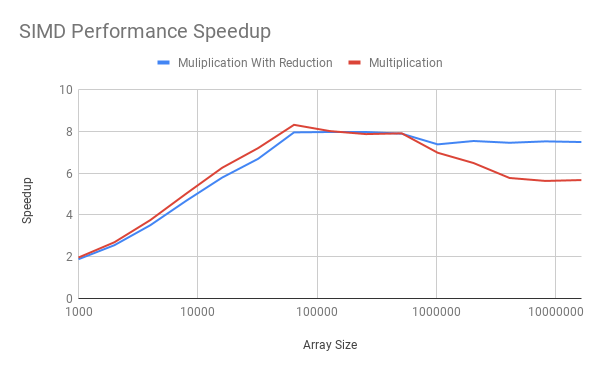
\includegraphics[width=\linewidth]{results}

  \item \textbf{Pattern Analysis} 
        The speedup varies considerably across array sizes, which is surprising at least
        for large values. I anticipated that small array sizes would have very inconsistent
        results and large values would tend towards some fixed values. In fact, we see that 
        the arraysize of around 100000 has the largest speedup gains and then the speedup
        gains decrease afterward. The speedup for the largest values
        settled around 5.5 for the array-by-array multiplication and around 7.5 for the 
        array-by-array reduction, both of which are surprising. 
        
        A naive guess for the speedup would predict a speedup of 4 for both pairs of algorithms, 
        since the SIMD programs are telling the processor to run four
        times as many computations for every computation in the non-SIMD programs. However,
        there are several reasons why the speedup might deviate from 4. 

        First, since the majority of the
        work in the SIMD programs is performed through assembly instructions, it might have
        significant performance gains by skipping the overhead involved in the higher level
        language of C++. These performance gains would obviously increase the speedup past
        the naive estimate of 4.
        
        As to why the reduction algorithm performs considerably better than the multiplication
        algorithm, one plausible explanation (offered by Professor Bailey) 
        is that the assembly instructions in the reduction algorithm involve one more 
        parallelized step: the summing into a register xmm2.
        

\end{enumerate}
\end{document}
